\subsubsection{GASNet-EX}
\paragraph{Overview} 

The Lightweight Communication and Global Address Space Support project (Pagoda)
is developing GASNet-EX, a portable high-performance communication layer
supporting multiple implementations of the Partitioned Global Address Space
(PGAS) model, including Pagoda's PGAS programming interface UPC++~\cite{Bachan:paw17}
 and the Legion Programing
System~\cite{bauer2012legion,legion-site} (WBS~2.3.1.08).

GASNet-EX's low-overhead communication mechanisms can maximize
injection rate and network utilization, tolerate latency through
overlap, streamline unpredictable communication events, minimize
synchronization, and efficiently support small- to medium-sized
messages arising in ECP applications.  GASNet-EX will enable the ECP
software stack to exploit the best-available communication mechanisms,
including novel features still under development by vendors.  The
GASNet-EX communications library and the PGAS models built upon it
offer a complementary, yet interoperable, approach to MPI with OpenMP,
enabling developers to focus their effort on optimizing
performance-critical communication.

We are co-designing GASNet-EX with the UPC++ development team with
additional input from the Legion and
(non-ECP) Cray Chapel~\cite{chapel-chapter,chapel-site} projects.

\paragraph{Key  Challenges}

Exascale systems will deliver exponential growth in on-chip parallelism and
reduced memory capacity per core, which will increase the need for strong
scaling and thus smaller communication events.  To scale well, Exascale
software needs to minimize the work performed by lightweight cores and avoid the
overhead of long, branchy serial code paths; it needs to support efficient
fine-grained communication.
These problems are exacerbated by application trends; many of the ECP applications require
adaptive meshes, sparse matrices,
or dynamic load balancing.
All of these point to the need for low-overhead communication mechanisms that
can maximize injection rate and network utilization, tolerate latency through
overlap, accommodate unpredictable communication events, minimize synchronization,
and efficiently support small- to medium-sized messages. The ECP software stack
needs to expose the best-available communication mechanisms, including novel
features being developed by the vendor community.

\paragraph{Solution Strategy}

The Global Address Space (GAS) model is a powerful means of addressing these
challenges and is critical in building other ECP programming systems,
libraries, and applications.  We use the term {\em GAS} for models that support
one-sided communication (including contiguous and non-contiguous remote put/get
operations and atomics). Many of these models also include support for remote function invocation.
GASNet-EX is a communications library that provides the foundation for implementing
GAS models, and is the successor to the widely-deployed GASNet library.
We are building on 15 years of experience with the GASNet~\cite{gasnet-spec,gasnet-site}
communication layer to provide production-quality implementations that include
improvements that address
technology trends and application experience.  

The goal of the GASNet-EX work is to provide a portable, high-performance GAS
communication layer for Exascale and pre-Exascale systems, to address the challenges
identified above.
GASNet-EX provides interfaces that efficiently match the RDMA capabilities of modern
inter-node network hardware and intra-node communication between distinct address spaces.
Interfaces for atomics and collectives are being developed to enable offload to current
and future network hardware with corresponding capabilities.
These design choices and their implementations provide the low-overhead communications
mechanisms required to address Exascale applications' requirements.


\paragraph{Recent Progress}

The 2017.6.0 release of GASNet-EX introduced three new features, known as ``New Active
Message Interfaces'', ``Immediate Operations'' and ``Local Completion''.  The 2017.12.0 release
introduced a new ``Remote Atomics'' feature, as well as ``Expanded VIS Interfaces''.  
These two releases contain network-independent
``reference'' implementations of these features, which provide implementations in terms of
the pre-existing functionality available in GASNet-EX on all networks.  While these
reference implementations are correct and functionally complete, they do not take advantage
of network-specific mechanisms.

The most recent work, present in the 2018.3.0 release, 
provides network-{\em specific} implementations of GASNet-EX's new features
for the Cray Aries network used in Cray XC-series systems.
Performance gains achieved include (1) Negotiated-Payload Active Messages improve
bandwidth of a ping-pong test by up to 14\%, (2) Immediate Operations reduce running time
of a synthetic benchmark by up to 93\%, (3) non-bulk RMA Put bandwidth is increased by up
to 32\%, (4) Remote Atomic performance is 70\% faster than the reference on a point-to-point
test and allows a hot-spot test to scale robustly, and (5) non-contiguous RMA interfaces
see up to 26\% speedups for an inter-node benchmark.  More complete details are
available in an LBNL Technical Report~\cite{gasnet-aries}.

\begin{figure}[htb]
 % \captionsetup{format=centeredCaption}
  \centering
  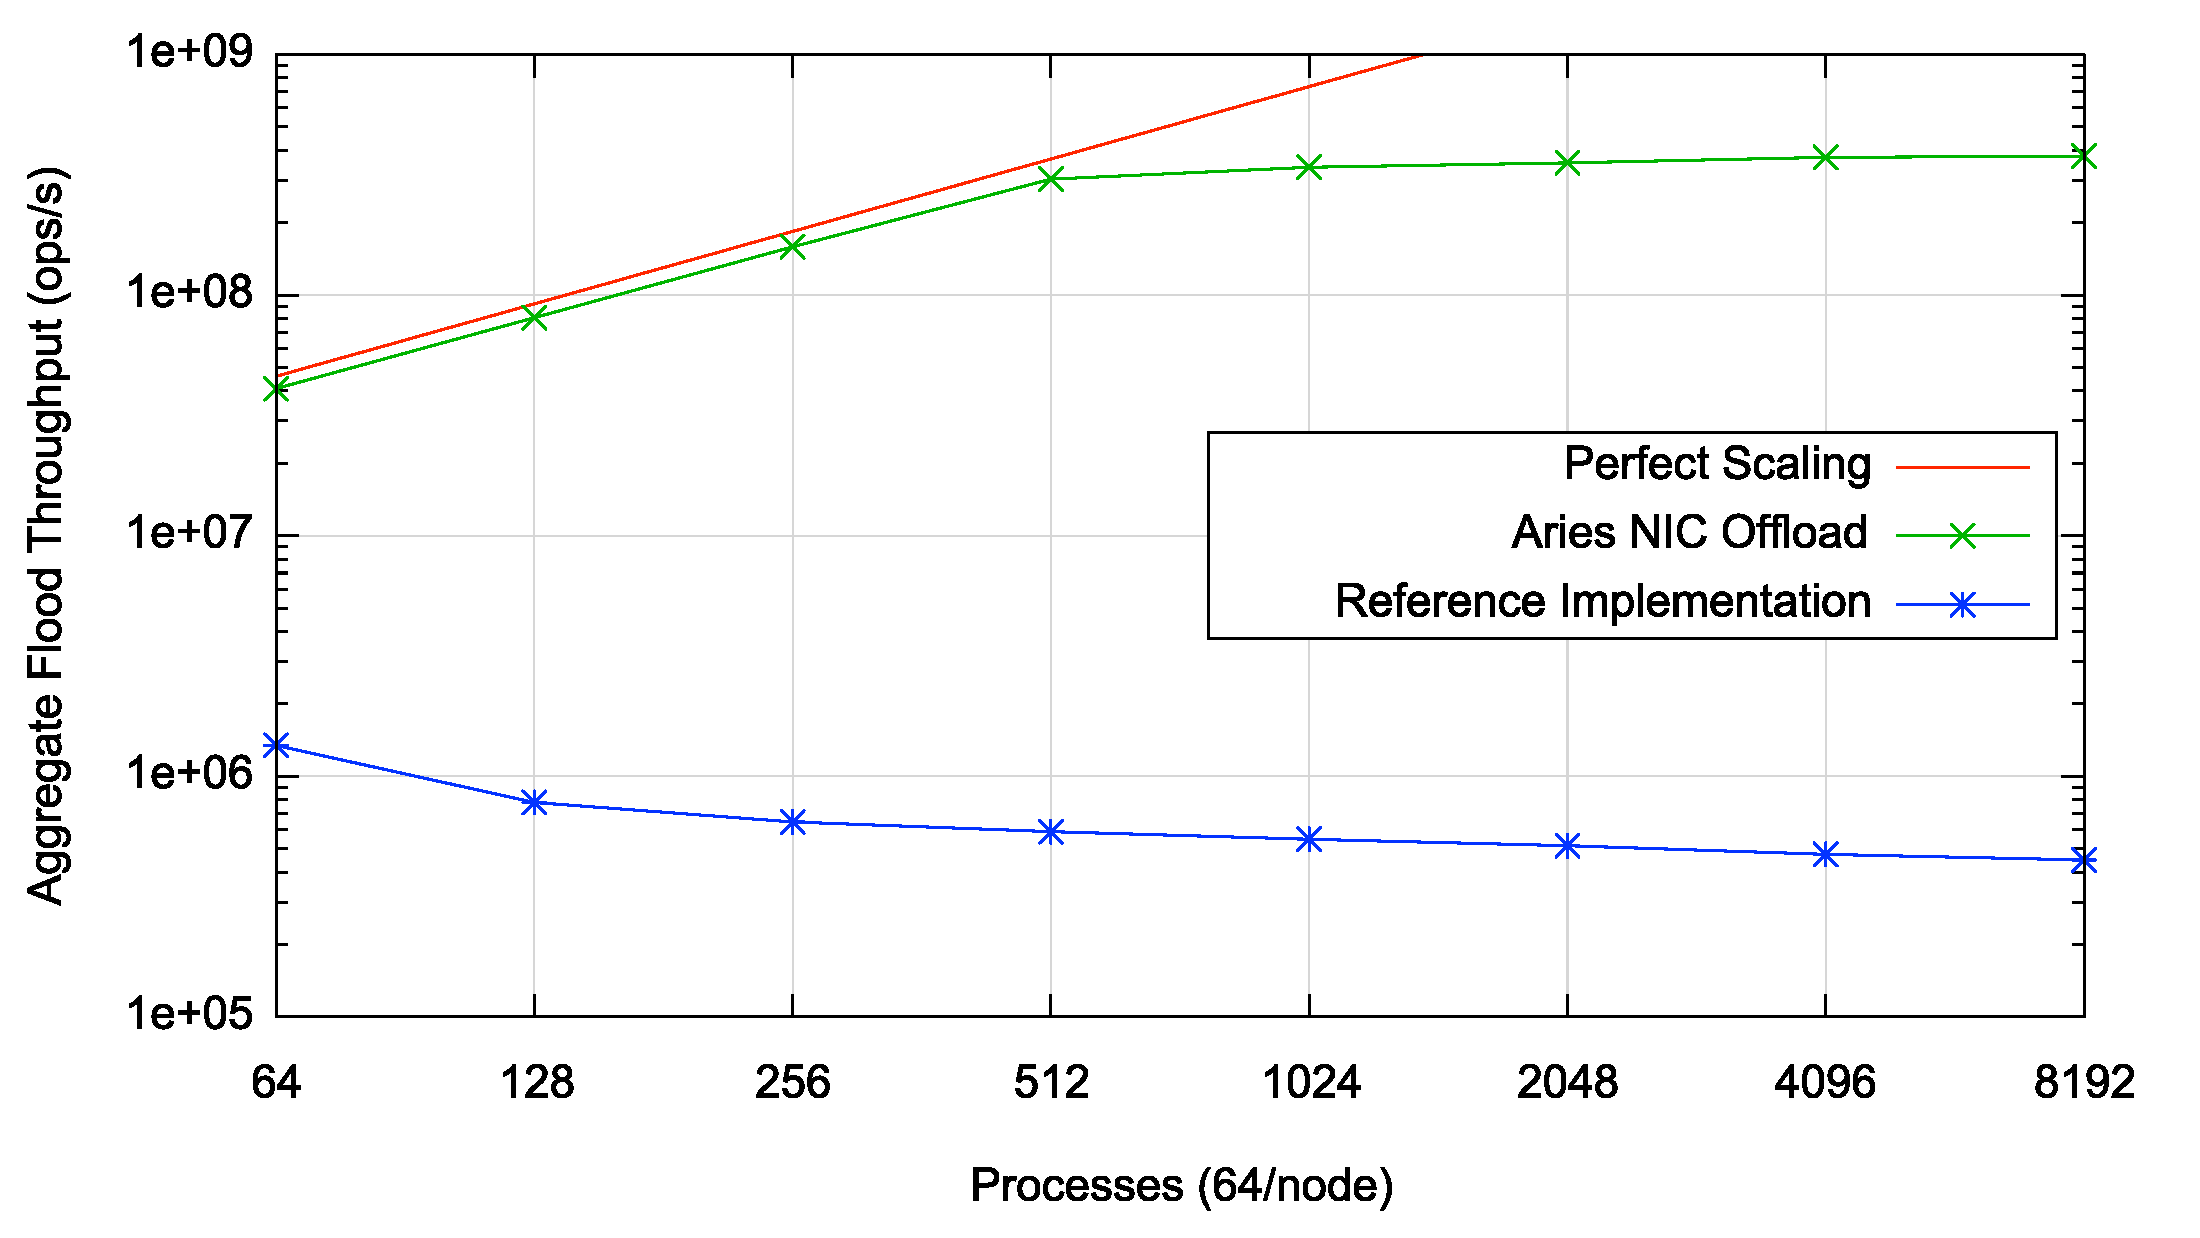
\includegraphics[width=\textwidth]{projects/2.3.1-PMR/2.3.1.14-UPCxx-GASNet/aries-fadd.pdf}
  \caption{\label{fig:aries-fadd}
           Weak Scaling of 64-bit Unsigned Integer Atomic Hot-Spot Test on ALCF's Theta}
\end{figure}

The Aries-specific implementation of remote atomics offloads most operations to
the Aries NIC, yielding a 1.7x reduction in latency, and greatly improved
scalability in a many-to-one atomics hot-spot test.
Figure~\ref{fig:aries-fadd} shows results on ALCF's Cray XC-40, Theta, for such
a benchmark in which all 64 cores on one or more compute nodes simultaneously
perform 64-bit unsigned integer \texttt{fetch-and-add} operations on a single location.
The figure shows the aggregate throughput as a function of the number
of processes.  The data shows that as the process count increases, the aggregate
performance of the reference implementation actually drops (due to overheads of
message reception dominating).  Meanwhile the performance of the Aries-specific
version rises steadily as the node count increases from 1 to 8 (64 to 512
processes), and continues to rise gradually from that point to the highest
concurrency measured (128 nodes = 8192 processes).  For comparison, the
``Perfect Scaling'' line (in red at the upper-left of the figure) shows the
throughput of a single-process run scaled by the process count.

\paragraph{Next Steps}

Our next efforts include:
\begin{enumerate}

\item \textbf{``Teams and Collectives''} are to be updated (both specification
and implementation) for new GASNet-EX interfaces to improve scalability and to
enable future offload efforts.

\item \textbf{``Dependent Operations''} are to be implemented, to permit client
runtimes to express ordered sequences of operations to be executed by GASNet-EX.

\end{enumerate}
